%%%%%%%%%%%%%%%%%%%%%%%%%%%%%%%%%%%%%%%%%
% Journal Article
% LaTeX Template
% Version 2.0 (February 7, 2023)
%
% This template originates from:
% https://www.LaTeXTemplates.com
%
% Author:
% Vel (vel@latextemplates.com)
%
% License:
% CC BY-NC-SA 4.0 (https://creativecommons.org/licenses/by-nc-sa/4.0/)
%
% NOTE: The bibliography needs to be compiled using the biber engine.
%
%%%%%%%%%%%%%%%%%%%%%%%%%%%%%%%%%%%%%%%%%

%----------------------------------------------------------------------------------------
%	PACKAGES AND OTHER DOCUMENT CONFIGURATIONS
%----------------------------------------------------------------------------------------

\documentclass[
	a4paper, % Paper size, use either a4paper or letterpaper
	10pt, % Default font size, can also use 11pt or 12pt, although this is not recommended
	unnumberedsections, % Comment to enable section numbering
	twoside, % Two side traditional mode where headers and footers change between odd and even pages, comment this option to make them fixed
]{LTJournalArticle}

\addbibresource{sample.bib} % BibLaTeX bibliography file

\runninghead{Apollo 13 Scouting} % A shortened article title to appear in the running head, leave this command empty for no running head

\footertext{\textit{Apollo 13 Scouting} (2025) Michel Bijnen} % Text to appear in the footer, leave this command empty for no footer text

\setcounter{page}{1} % The page number of the first page, set this to a higher number if the article is to be part of an issue or larger work

%----------------------------------------------------------------------------------------
%	TITLE SECTION
%----------------------------------------------------------------------------------------

\title{Programma Apollo 13} % Article title, use manual lines breaks (\\) to beautify the layout

% Authors are listed in a comma-separated list with superscript numbers indicating affiliations
% \thanks{} is used for any text that should be placed in a footnote on the first page, such as the corresponding author's email, journal acceptance dates, a copyright/license notice, keywords, etc
\author{%
	Michel Bijnen
}

% Affiliations are output in the \date{} command
% \date{\footnotesize\textsuperscript{\textbf{1}}Scouting Mierlo-Hout Welpen}

% Full-width abstract
\renewcommand{\maketitlehookd}{%
	\begin{abstract}
		\noindent De groep simuleert dat ze de controlekamer van een missie van Apollo 13 zijn. De groep bepaalt zelf welke        van de volgende rollen ze willen zijn:
            \begin{itemize}
                \item Missie directeur
                \item Communicatie (CAPCOM)
                \item Staff
                \item Incident manager
                \item Navigatie expert (FIDO)
                \item Gezondheid expert (EECOM)
                \item Engineering expert
                \item Communicatie expert (INCO)
            \end{itemize}
            Gebaseerd op deze rollen krijgt iedereen een uitleg wat ze moeten doen. \\
            \noindent Benodigdheden:
            \begin{itemize}
                \item Programma + laptop waar de mission director aan kan
                \item Beamer
                \item Handleidingen voor expert
                \item Meerdere A6 incident report cards
                \item Pennen en notitiemateriaal
                \item Tafels en stoelen
                \item 6 titel bordjes (4 voor de experts, 1 voor de directeur, 1 voor communicatie, en 1 voor de incident managers)
            \end{itemize}
	\end{abstract}
}

%----------------------------------------------------------------------------------------

\begin{document}

\maketitle % Output the title section

%----------------------------------------------------------------------------------------
%	ARTICLE CONTENTS
%----------------------------------------------------------------------------------------

\section{Introductie}

Apollo 13 was een beroemde Amerikaanse ruimtemissie gelanceerd door NASA in 1970. Deze missie was oorspronkelijk gepland als de derde bemande maanlanding van het Apollo-programma. Echter, Apollo 13 kreeg wereldwijde aandacht vanwege een ernstige technische storing aan boord van het ruimtevaartuig. Terwijl de bemanning, bestaande uit astronauten James Lovell, John Swigert en Fred Haise, onderweg was naar de maan, trad er een explosie op in een van de zuurstoftanks. Dit leidde tot een noodsituatie waarin de bemanning moest improviseren om veilig terug te keren naar de aarde. Het was tijdens deze kritieke momenten dat astronaut Jim Lovell de beroemde woorden uitsprak: "Houston, we have a problem." Deze zin markeerde het begin van een intensieve samenwerking tussen de bemanning en het grondcontroleteam in Houston, Texas, terwijl ze creatieve oplossingen bedachten om de astronauten veilig naar huis te brengen. Apollo 13 blijft een inspirerend voorbeeld van vastberadenheid en teamwork in de ruimtevaartgeschiedenis.

\begin{figure}
	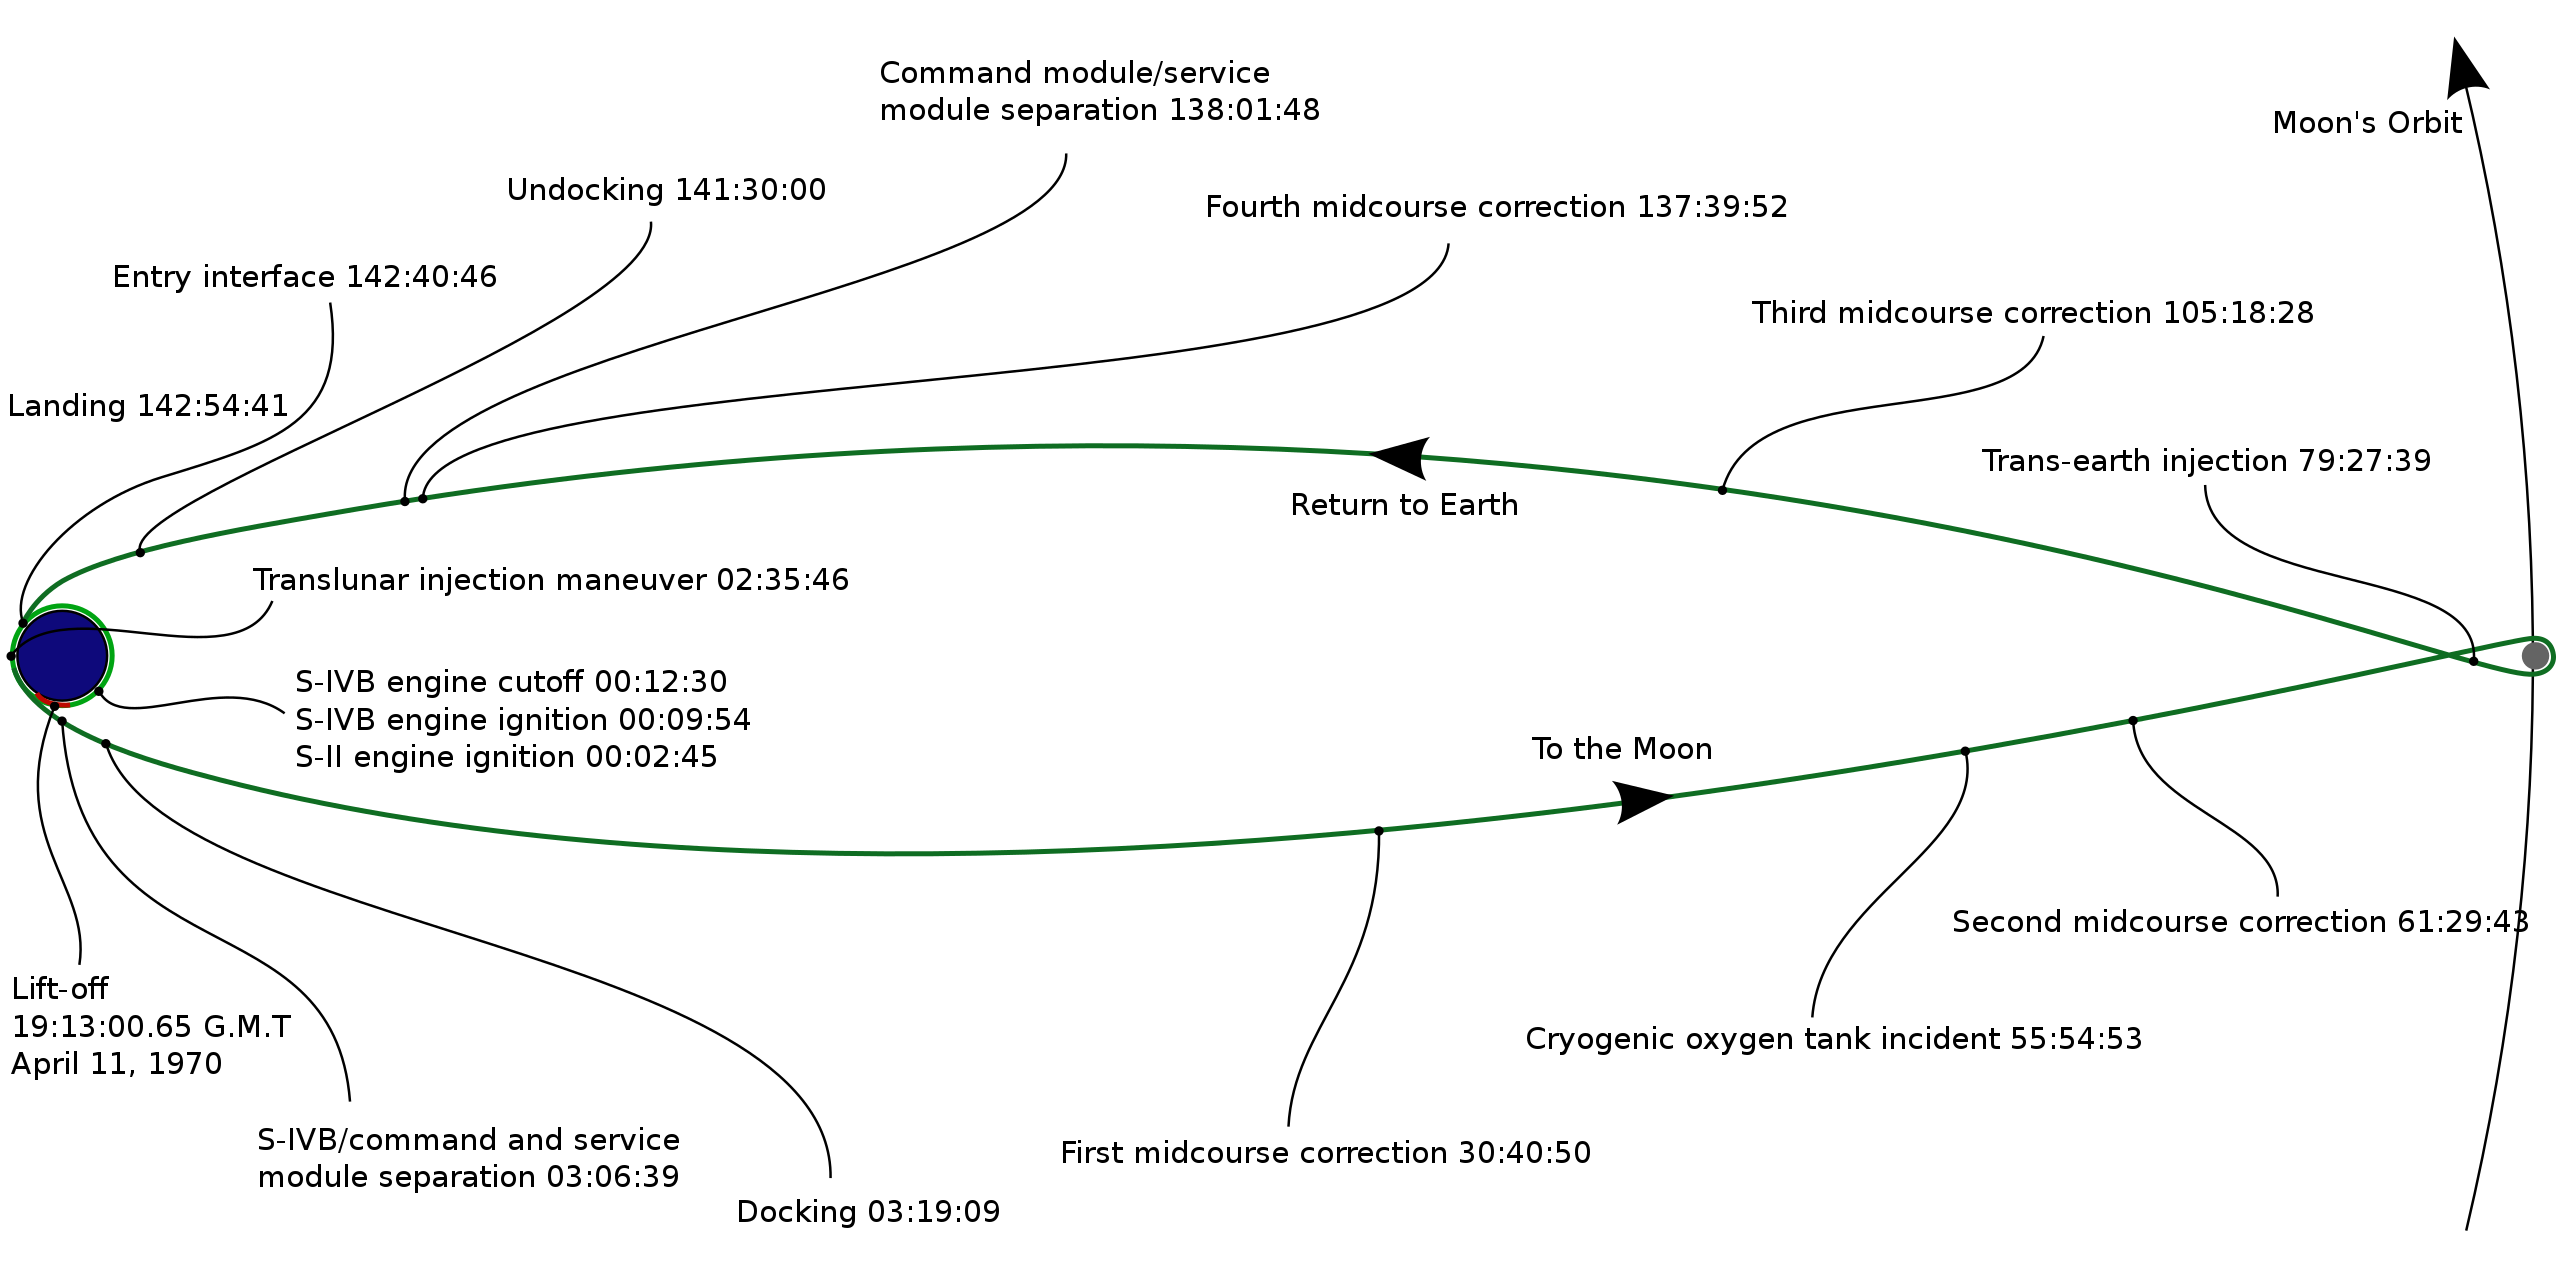
\includegraphics[width=\linewidth]{Figures/Timeline.png}
	\caption{Apollo 13 tijdlijn.}
	\label{fig:timeline}
\end{figure}

Dit spel is een coöperatief spel, wat betekent dat de groep als geheel kan winnen of verliezen. Het doel van dit spel is om de samenwerking binnen de groep te bevorderen. Aanvankelijk worden er enkele uitdagingen aan de groep gepresenteerd om hen vertrouwd te maken met de basisprincipes van het spel. Na verloop van tijd worden er steeds meer uitdagingen toegevoegd, waardoor de situatie steeds chaotischer wordt. Als de groep kalm kan blijven en in staat is om binnen een bepaalde tijd oplossingen te vinden voor de problemen door goed samen te werken, zal de missie succesvol worden afgerond.

\subsection{Spelverloop}
Tijdens dit spel simuleert de groep mission control tijdens de Apollo 13 vlucht. Het spel heeft een variabele duur, maar het wordt aanbevolen om ongeveer één uur te spelen. Samen met de opzettijd, het verhaal voorafgaand aan het spel, het afsluitende verhaal en de uitleg zal de totale tijdsinvestering ongeveer anderhalf tot twee uur bedragen. Twee van de spelleiders vervullen de rol van astronauten. Zij bepalen welke uitdagingen aan de groep worden gegeven, de snelheid waarmee dit gebeurt, en dus ook de moeilijkheidsgraad van de opdrachten. De uitdagingen zijn afzonderlijk uitgewerkt, waarbij sommige verplicht zijn om het verhaal van Apollo 13 en de belangrijkste gebeurtenissen daadwerkelijk te laten plaatsvinden.

\begin{figure}
	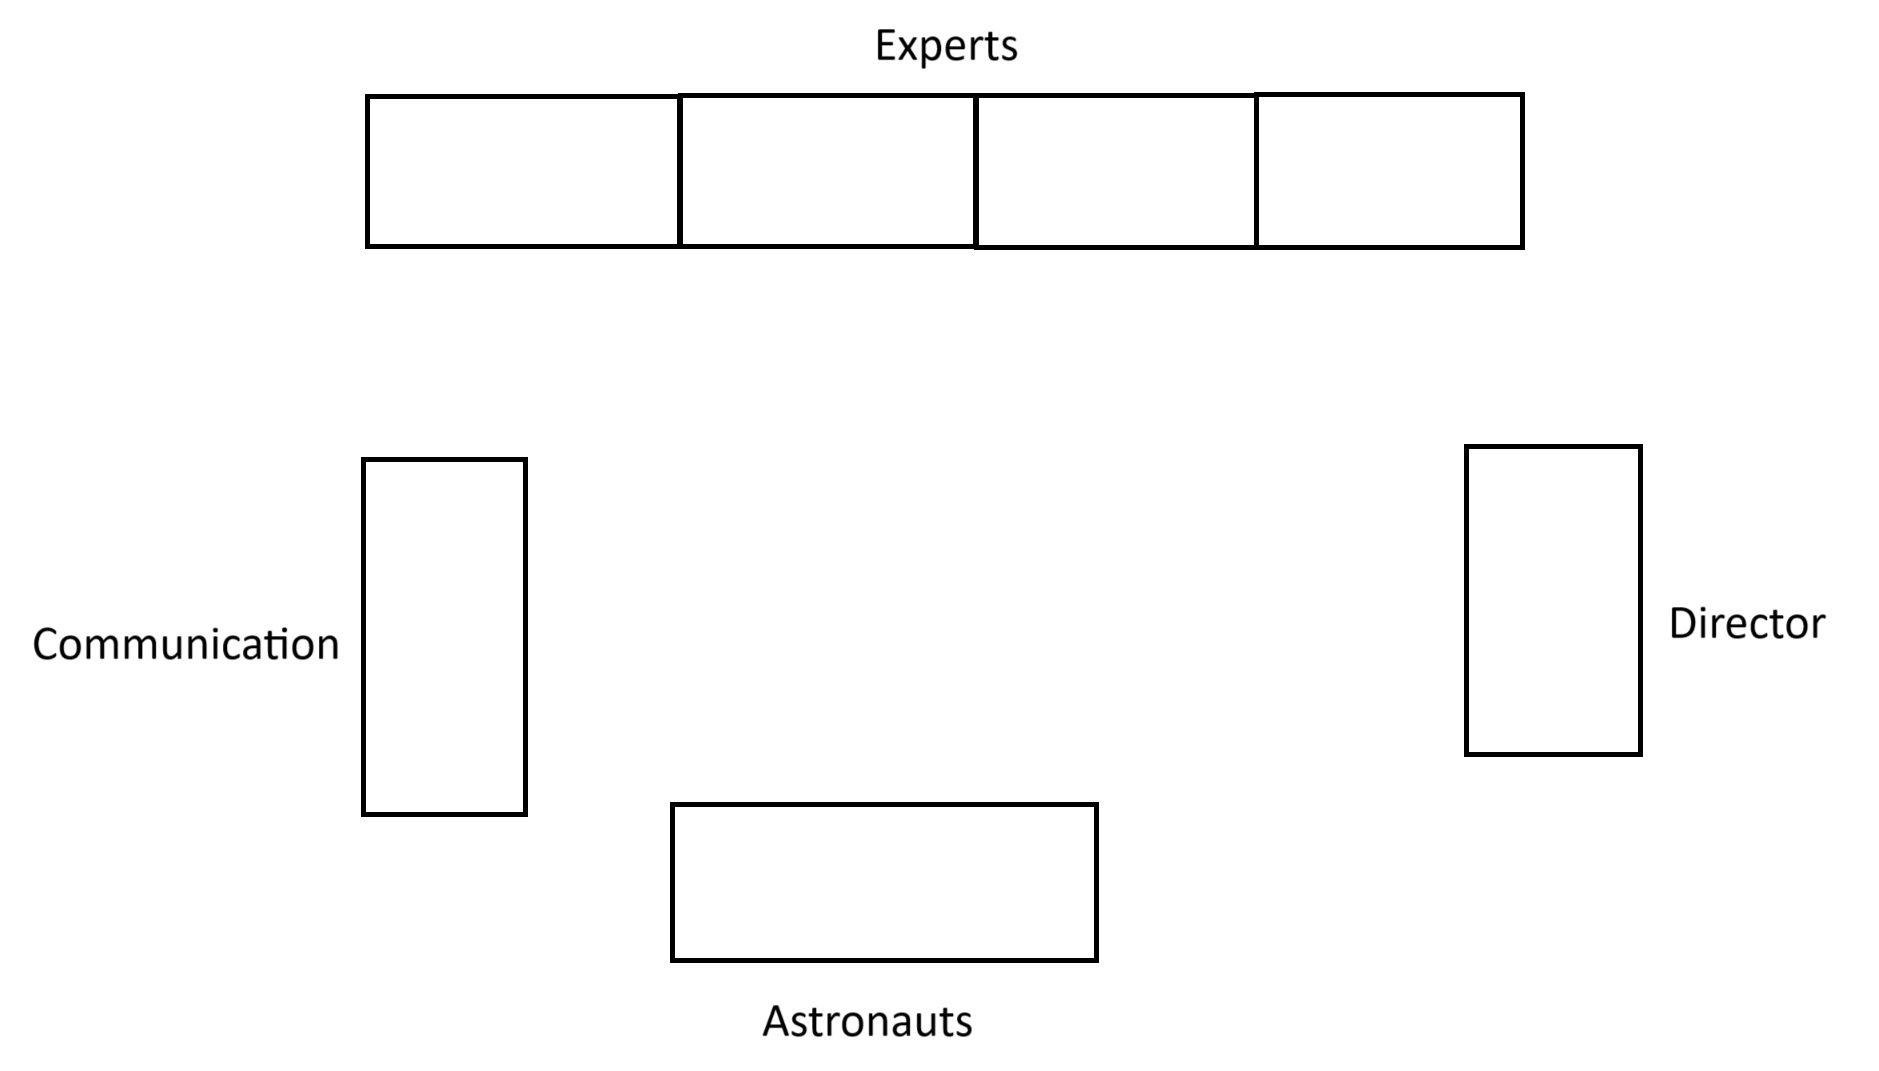
\includegraphics[width=\linewidth]{Figures/Layout.jpg}
	\caption{Indeling van de kamer.}
	\label{fig:timeline}
\end{figure}

%------------------------------------------------

\section{Rollen}

\subsection{Missie directeur}

De rol van directeur is een van de meest cruciale rollen in het spel. Deze persoon is verantwoordelijk voor het behouden van een overzicht van de gebeurtenissen en het bewaken van het grotere geheel. Tevens heeft de directeur de controle over wat er op het grote scherm wordt weergegeven en kan hij/zij schakelen tussen de volgende schermen:
\begin{itemize}
    \item Navigatiekaart en theoretische locatie van het schip.
    \item Medische sensoren, zoals de hartslag en bloeddruk van de astronauten.
    \item De status van het ruimtevaartuig.
\end{itemize}
Omdat de directeur over deze controles beschikt, is het van essentieel belang dat hij/zij voortdurend alert is op eventuele problemen. Bovendien draagt de directeur, voor het verloop van het verhaal, de eindverantwoordelijkheid voor het succesvol laten verlopen van de missie.

\subsection{Incident manager}
De incident managers zijn verantwoordelijk dat de incidenten opgelost worden. Zij zijn ook de eerste personen waar een incident bij aan komt. Zij sturen het incident dan naar 1 van de experts die advies geven over hoe het probleem opgelost moet worden. Daarna kan de incident report weer terug naar CAPCOM. Wanneer een incident afgerond is, gaat de kaart weer terug naar de incident managers. Hierdoor kunnen zij een logboek bijhouden van incidenten die in het verleden zijn gebeurd. Dit zorgt er weer voor dat bepaalde herhaalde incidenten sneller opgelost kunnen worden.

\subsection{Communicatie}

Het communicatieteam fungeert als het primaire aanspreekpunt voor de astronauten. Zij zijn verantwoordelijk voor het ontvangen van vragen en het doorgeven van problemen. De astronauten zullen op geen enkele manier vragen beantwoorden en zullen geen acties ondernemen op basis van suggesties van andere teamleden. Alle problemen komen eerst bij het communicatieteam binnen, waar ze worden gedocumenteerd. Vervolgens beoordeelt dit team onmiddellijk de urgentie van de uitdagingen voordat ze worden doorgegeven aan de experts voor verdere behandeling.

\subsection{Expert team}

Er zijn vier experts, elk met een specifieke rol en bijbehorende informatie. Elke expert heeft een aparte set gegevens, die voorafgaand aan de simulatie aan hen wordt verstrekt. Deze informatie is vertrouwelijk en mag niet worden gelezen door andere teamleden. De gegevens bevatten gedetailleerde oplossingen voor de uitdagingen, evenals stappen die moeten worden gecontroleerd om de uitdagingen met succes op te lossen. Het expertteam ontvangt deze specifieke informatie bij de start van het spel om hun taken uit te voeren.

\subsubsection{Navigatie expert}
De navigatie-expert heeft de verantwoordelijkheid om de trajectorie van het ruimtevaartuig te beheren en ervoor te zorgen dat het op koers blijft door regelmatig de navigatiekaart te raadplegen en eventuele afwijkingen op te lossen. Het grootste deel van de navigatie gebeurt met behulp van een sterrenkaart, die de posities van specifieke sterren volgt om de locatie nauwkeurig te bepalen. De navigatie-uitdagingen zijn gebaseerd op het gebruik van deze sterrenkaart, en ze omvatten ook aspecten met betrekking tot de snelheid van de raket.

\subsubsection{Gezondheid expert}
De gezondheidsexpert draagt de verantwoordelijkheid voor het monitoren van de gezondheidstoestand van de astronauten. Dit omvat voortdurende observatie van de bloeddruk en hartslag om ervoor te zorgen dat de astronauten in staat zijn hun taken adequaat uit te voeren. Bovendien is de gezondheidsexpert belast met het controleren van de luchtkwaliteit in de cockpit, waaronder het handhaven van een voldoende hoog zuurstofniveau om de gezondheid en prestaties van de astronauten te waarborgen.

\subsubsection{Engineering expert}
De engineeringexpert heeft de verantwoordelijkheid om de status van het ruimtevaartuig in de gaten te houden. Deze expert is belast met het oplossen van problemen met alle systemen en componenten die kunnen falen aan boord van het ruimtevaartuig. Dit omvat niet alleen het handhaven van de integriteit van de romp van het ruimtevaartuig maar ook het zorgen voor de goede werking van verschillende interne apparatuur en systemen. De engineeringexpert is essentieel om ervoor te zorgen dat het ruimtevaartuig in optimale staat blijft en veilig kan blijven functioneren.

\subsubsection{Communicatie expert}
De communicatie-expert draagt de verantwoordelijkheid voor alle aspecten van communicatie aan boord van het ruimtevaartuig. Storingen kunnen vaak de communicatie tussen het ruimtevaartuig en missiecontrole verstoren, daarom moet de communicatie-expert analoge signalen naar het ruimtevaartuig verzenden zodat eventuele communicatieproblemen kunnen worden opgelost. Bovendien is de communicatie-expert verantwoordelijk voor het informeren van de groep wanneer directe communicatie niet mogelijk is, bijvoorbeeld wanneer het ruimtevaartuig zich achter de maan bevindt. Deze rol is cruciaal om ervoor te zorgen dat de communicatie te allen tijde wordt gehandhaafd en eventuele problemen snel worden opgelost.

\subsection{Staff}
De stafleden zijn algemene teamleden die verantwoordelijk zijn voor het ontvangen van uitdagingen van teamleden en ervoor zorgen dat deze worden opgelost. Ze zijn flexibel en kunnen overal bijspringen om hulp te bieden, maar hun hoofdtaak is gericht op het coördineren van de uitdagingen en ervoor te zorgen dat deze worden doorgegeven aan de juiste expert. Op deze manier dragen ze bij aan het handhaven van de communicatie met de astronauten door ervoor te zorgen dat de problemen snel en effectief worden opgelost.

\newpage
\appendix

\section{Story}
This appendix contains all story challenges that have to happen at a certain point during the mission.

\vspace{1cm}
\subsection{Motoruitval}
T+00:00:00

\subsubsection{Probleem}
Motor 5 valt uit

\subsubsection{Wat ons opvalt}
Rood lampje van 'motor 5' springt aan.

\subsubsection{Wat wij mogelijk kunnen vinden}
De motor lijkt gestopt te zijn.

\subsubsection{Wat er gebeurt als het niet snel genoeg opgelost wordt}
Niks, er is genoeg stuwkracht.

\subsubsection{Wat te doen om het op te lossen}
De vier motoren is genoeg stuwkracht om de raket uit orbit te krijgen.
\vspace{1cm}
\subsection{Vocht en condens probleem}
T+00:06:00

\subsubsection{Probleem}
Door een verhoogde hoeveelheid condens, is de kans groter dat er kortsluiting komt.

\subsubsection{Wat ons opvalt}
Vocht en condens in de capsule die zich verzamelen op de apparatuur en oppervlakte.

\subsubsection{Wat wij mogelijk kunnen vinden}

\subsubsection{Wat er gebeurt als het niet snel genoeg opgelost wordt}
Probleem 'zuurstof tank explosie'.

\subsubsection{Wat te doen om het op te lossen}
Handmatig wegpoetsen van de handdoeken, maar echter niet genoeg.
\vspace{1cm}
\subsection{Zuurstof tank explosie}
T+00:12:00

\subsubsection{Probleem}
Door kortsluiting ontploft de zuurstoftank.

\subsubsection{Wat ons opvalt}
\begin{itemize}
    \item Knalgeluid
    \item Zuurstoftank 2 waarschuwingslampje
\end{itemize}

\subsubsection{Wat wij mogelijk kunnen vinden}
Na onderzoek, zien we dat er lucht de ruimte in ventileert.

\subsubsection{Wat er gebeurt als het niet snel genoeg opgelost wordt}
De CM wordt onleefbaar, wat resulteert in de astronauten sterven.

\subsubsection{Wat te doen om het op te lossen}
\begin{itemize}
    \item Alle niet essentiële systemen moeten uitgeschakeld worden
    \item Bemanning moet naar de LM verplaatsen
\end{itemize}

% \subsection{Zuurstof tank explosie}

\subsubsection{Probleem}
Probleem

\subsubsection{Wat ons opvalt}
Appels

\subsubsection{Wat wij mogelijk kunnen vinden}
Appels

\subsubsection{Wat er gebeurt als het niet snel genoeg opgelost wordt}
Appels

\subsubsection{Wat te doen om het op te lossen}
Appels
\vspace{1cm}
\subsection{Navigatieproblemen}

\subsubsection{Probleem}
Navigatiesystemen werken niet meer.

\subsubsection{Wat ons opvalt}
Navigatie apparatuur lijkt foutief te zijn.

\subsubsection{Wat wij mogelijk kunnen vinden}
-

\subsubsection{Wat er gebeurt als het niet snel genoeg opgelost wordt}
Capsule raakt uit koers.

\subsubsection{Wat te doen om het op te lossen}
Met behulp van de sterrenkaart en sterren aangeven waar de raket heen moet vliegen.
\vspace{1cm}
\subsection{Opstapeling CO2 in de capsule}

\subsubsection{Probleem}
Tekort aan O2 en opstapeling van CO2 door te weinig filters in de capsule.

\subsubsection{Wat ons opvalt}
Astronauten worden suf, gapen veel, reageren traag, vitale functies wijken af.

\subsubsection{Wat wij mogelijk kunnen vinden}
Vitale functies gaan achteruit.

\subsubsection{Wat er gebeurt als het niet snel genoeg opgelost wordt}
Overlijden van astronauten.

\subsubsection{Wat te doen om het op te lossen}
Geïmproviseerde luchtfilters maken van ducttape, sokken, slangen van de pakken, karton, plastic hoezen en instructies van de grondleiding.
\vspace{1cm}
\subsection{Kou in de capsule}

\subsubsection{Probleem}
Koud in de capsule.

\subsubsection{Wat ons opvalt}
Astronauten blazen rook ( lucht uit hun mond), klappertanden, condens op de ramen en apparatuur. rillen enz

\subsubsection{Wat wij mogelijk kunnen vinden}
-

\subsubsection{Wat er gebeurt als het niet snel genoeg opgelost wordt}
Astronauten raken onderkoeld, functioneren minder goed, raken uitgeput. En uiteindelijk worden ze ziek.

\subsubsection{Wat te doen om het op te lossen}
\begin{itemize}
    \item Zoveel mogelijk lagen kleren aan trekken over elkaar
    \item Zoveel mogelijk in hun slaapzakken gaan liggen.
\end{itemize}
\vspace{1cm}
\subsection{Slechte hygiëne en ongemak}

\subsubsection{Probleem}
Astronauten voelen zich vies en ongemakkelijk door beperking stroom en water en hergebruik urinezakken.

\subsubsection{Wat ons opvalt}
Astronauten lijken wat depressief te raken en hun moralen en fysieke conditie gaat achteruit.

\subsubsection{Wat wij mogelijk kunnen vinden}
-

\subsubsection{Wat er gebeurt als het niet snel genoeg opgelost wordt}
Astronauten hebben stress, worden ziek waardoor ze minder inzetbaar zijn.

\subsubsection{Wat te doen om het op te lossen}
Alle suggesties zijn mogelijk.
\vspace{1cm}
\subsection{Urineweginfectie}

\subsubsection{Probleem}
Een astronaut krijgt een urineweginfectie.
Door slechte hygiëne en te weinig vocht om te drinkendoordat er een vochtbeperking is ingesteld en door de koude omgeving in de capsule

\subsubsection{Wat ons opvalt}
Astronaut gaat conditioneel achteruit, koorts, pijn bij plassen en veel kleine beetjes plassen.

\subsubsection{Wat wij mogelijk kunnen vinden}
-

\subsubsection{Wat er gebeurt als het niet snel genoeg opgelost wordt}
Astronaut word steeds zieker als de urineweginfectie niet wordt behandeld, word septisch en uiteindelijk komt hij te overlijden.

\subsubsection{Wat te doen om het op te lossen}
\begin{itemize}
    \item Rust
    \item Antibiotica innemen
\end{itemize}
 Niet echt een oplossing hiervoor ivm beperkte medische maatregelen in de capsule.
 Tijdelijke oplossing tot terug keer op aarde: 
 - meer vocht tot zich nemen
 -Rust en minimale inspanning
 - pijnstillers
\vspace{1cm}
\subsection{Beperkte energie voorziening}

\subsubsection{Probleem}
Beperkte energievoorzieningen in de capsule

\subsubsection{Wat ons opvalt}
De stroom loopt te snel leeg in de LM.


\subsubsection{Wat wij mogelijk kunnen vinden}
-

\subsubsection{Wat er gebeurt als het niet snel genoeg opgelost wordt}
Geen systemen zorgt ervoor dat communicatie, navigatie, en levensondersteuning niet mogelijk zijn wat resulteert in dood.

\subsubsection{Wat te doen om het op te lossen}
Zo veel mogelijk systemen uitschakelen.
\vspace{1cm}
\subsection{Slechte slaapomstandigheden}

\subsubsection{Probleem}
Bemanning slaapt slecht door de kou en krappe ruimte.

\subsubsection{Wat ons opvalt}
Door het slaapgebrek raakten de astronauten fysiek en mentaal uitgeput

\subsubsection{Wat wij mogelijk kunnen vinden}
-

\subsubsection{Wat er gebeurt als het niet snel genoeg opgelost wordt}
Door de verminderde concentratie besluitvaardigheid worden er grote fouten gemaakt

\subsubsection{Wat te doen om het op te lossen}
Ze wisselden rustperiodes af, maar veel astronauten gaven toe dat ze nauwelijks echte slaap kregen.
% \vspace{1cm}
% \input{Challenges/Story/zonnescherm}

\clearpage
\section{Extra challenges}
This appendix contains all possible challenges which can be picked from as 'random' events.

\vspace{1cm}
\subsection{Piepend geluid}

\subsubsection{Probleem}
Er klinkt een constant piepend geluid in de capsule.

\subsubsection{Wat ons opvalt}
De astronauten melden een irriterend geluid dat hun concentratie beïnvloed.

\subsubsection{Wat wij mogelijk kunnen vinden}
De piep lijkt afkomstig te zijn van een defecte sensor of luidspreker.

\subsubsection{Wat er gebeurt als het niet snel genoeg opgelost wordt}
De astronauten raken afgeleid, wat de efficiëntie van andere taken vermindert.

\subsubsection{Wat te doen om het op te lossen}
Identificeer de bron van het geluid door systemen één voor één te testen en herstart de defecte componenten.
\vspace{1cm}
\subsection{Boordcomputer kapot}

\subsubsection{Probleem}
De boordcomputer functioneert niet naar behoren.

\subsubsection{Wat ons opvalt}
Schermen reageren traag en geven foutmeldingen.

\subsubsection{Wat wij mogelijk kunnen vinden}
-

\subsubsection{Wat er gebeurt als het niet snel genoeg opgelost wordt}
Navigatie en systeemcontrole worden ernstig belemmerd.

\subsubsection{Wat te doen om het op te lossen}
Herstart de boordcomputer.
\vspace{1cm}
\subsection{Stoel opengescheurd}

\subsubsection{Probleem}
Een stoel in de capsule scheurt open.

\subsubsection{Wat ons opvalt}
Een astronaut meldt ongemak en losse materialen zweven rond.

\subsubsection{Wat wij mogelijk kunnen vinden}
-

\subsubsection{Wat er gebeurt als het niet snel genoeg opgelost wordt}
Probleem 'slechte slaapomstandigheden'.

\subsubsection{Wat te doen om het op te lossen}
Gebruik ducttape om de stoel tijdelijk te repareren.
\vspace{1cm}
\subsection{Communicatie problemen}

\subsubsection{Probleem}
Kapotte antenne

\subsubsection{Wat ons opvalt}
Rood lampje 'communicatie' brandt. 

\subsubsection{Wat wij mogelijk kunnen vinden}
Na verloop van tijd steeds slechtere communicatie met het grondpersoneel doordat er na een tijdje berichten terug komen of juist helemaal niks terug komt.

\subsubsection{Wat er gebeurt als het niet snel genoeg opgelost wordt}
Sommige berichten van CAPCOM komen niet door naar de astronauten.

\subsubsection{Wat te doen om het op te lossen}
\begin{itemize}
    \item Maak gebruik laagfrequentie antenne
    \item Capsule moet worden gedraaid om de antenne in een goede positie te krijgen
\end{itemize}
\vspace{1cm}
\subsection{Vertraging communicatie}

\subsubsection{Probleem}
Berichten tussen CAPCOM en de capsule worden vertraagd.

\subsubsection{Wat ons opvalt}
Antwoorden van de astronauten komen later binnen dan normaal.

\subsubsection{Wat wij mogelijk kunnen vinden}
Interferentie door externe factoren of softwarefouten.

\subsubsection{Wat er gebeurt als het niet snel genoeg opgelost wordt}
Kritieke communicatie wordt vertraagd, wat beslissingen kan vertragen.

\subsubsection{Wat te doen om het op te lossen}
Restart communicatieapparatuur.
\vspace{1cm}
\subsection{Vertraging computer systemen}

\subsubsection{Probleem}
De computer systemen werken vertraagd.

\subsubsection{Wat ons opvalt}
Reacties van het systeem duren langer dan normaal.

\subsubsection{Wat wij mogelijk kunnen vinden}
Overbelasting van de boordcomputer.

\subsubsection{Wat er gebeurt als het niet snel genoeg opgelost wordt}
Kritieke processen zoals navigatie of levensondersteuning worden vertraagd.

\subsubsection{Wat te doen om het op te lossen}
Herstart boordcomputer.
\vspace{1cm}
\subsection{Drinkwater vies}

\subsubsection{Probleem}
Kapotte drinkwater filter.

\subsubsection{Wat ons opvalt}
Drinkwater smaakt vies.

\subsubsection{Wat wij mogelijk kunnen vinden}
\begin{itemize}
    \item Drinkwater ziet bruin en proeft naar ijzer.
    \item Na pH test: pH waarde van 4.
\end{itemize}

\subsubsection{Wat er gebeurt als het niet snel genoeg opgelost wordt}
Dan krijgen de astronauten geen of vervuild water en krijgen ze lichamelijke klachten. Probleem 'Slechte hygiëne en ongemak'.

\subsubsection{Wat te doen om het op te lossen}
Waterfilter vervangen.
\vspace{1cm}
\subsection{Film camera kapot}

\subsubsection{Probleem}
De filmcamera functioneert niet meer.

\subsubsection{Wat ons opvalt}
De beelden komen met schade op de filmrol.

\subsubsection{Wat wij mogelijk kunnen vinden}
-

\subsubsection{Wat er gebeurt als het niet snel genoeg opgelost wordt}
Geen goede beelden worden gemaakt.

\subsubsection{Wat te doen om het op te lossen}
Vervang filmrol.
\vspace{1cm}
\subsection{Geen films}

\subsubsection{Probleem}
Er is geen toegang meer tot de films aan boord.

\subsubsection{Wat ons opvalt}
Astronauten kunnen geen films bekijken tijdens rustperiodes.

\subsubsection{Wat wij mogelijk kunnen vinden}
Een defecte opslagmodule.

\subsubsection{Wat er gebeurt als het niet snel genoeg opgelost wordt}
De moreel van de astronauten gaat omlaag, wat hun prestaties kan beïnvloeden.

\subsubsection{Wat te doen om het op te lossen}
\begin{itemize}
    \item Muziek luisteren als alternatief.
    \item De film digitaal versturen via de antenne (kost tijd, waar geen communicatie mogelijk is).
\end{itemize}
\vspace{1cm}
\subsection{Geuren oplosmiddelen en smeermiddelen}

\subsubsection{Probleem}
Een sterke geur van oplosmiddelen verspreidt zich in de capsule.

\subsubsection{Wat ons opvalt}
Astronauten melden een irriterende geur en lichte hoofdpijn.

\subsubsection{Wat wij mogelijk kunnen vinden}
Een lekkage in een onderhoudscompartiment.

\subsubsection{Wat er gebeurt als het niet snel genoeg opgelost wordt}
De luchtkwaliteit verslechtert, wat gezondheidsproblemen kan veroorzaken. Probleem 'Slechte hygiëne en Ongemakken'.

\subsubsection{Wat te doen om het op te lossen}
Sluit het lekkende compartiment af met ducttape.
\vspace{1cm}
\subsection{Lampje kapot}

\subsubsection{Probleem}
Een intern verlichtingslampje brandt niet meer.

\subsubsection{Wat ons opvalt}
Minder licht in de capsule.

\subsubsection{Wat wij mogelijk kunnen vinden}
Een defect peertje.

\subsubsection{Wat er gebeurt als het niet snel genoeg opgelost wordt}
Niks

\subsubsection{Wat te doen om het op te lossen}
Vervang het lampje met een reservelampje.
\vspace{1cm}
\subsection{Verloren pen}

\subsubsection{Probleem}
Een pen is kwijtgeraakt in de capsule.

\subsubsection{Wat ons opvalt}
Een astronaut meldt dat een schrijfobject niet kan worden gevonden.

\subsubsection{Wat wij mogelijk kunnen vinden}
-

\subsubsection{Wat er gebeurt als het niet snel genoeg opgelost wordt}
Niks.

\subsubsection{Wat te doen om het op te lossen}
Gebruik een pen van een andere astronaut.
\vspace{1cm}
\subsection{Sensorfout}

\subsubsection{Probleem}
Een van de sensoren is kapot.

\subsubsection{Wat ons opvalt}
Lampje van dat systeem gaat branden.

\subsubsection{Wat wij mogelijk kunnen vinden}
Niets mis met dat systeem.

\subsubsection{Wat er gebeurt als het niet snel genoeg opgelost wordt}
Onjuiste informatie kan resulteren in verkeerde beslissingen die genomen worden.

\subsubsection{Wat te doen om het op te lossen}
Herstart dat specifieke systeem en controleer de bekabeling.
\setcounter{page}{1}
\section{Skills}

\subsection{Missie Directeur}
\textit{Max 1 persoon}
\begin{itemize}
    \item Communicatie
    \item Besluitvorming
    \item Teamcoördinatie
    \item ProbleemAnalyse
\end{itemize}

\subsection{Incident Manager}
\textit{Advies: 2 personen}
\begin{itemize}
    \item Probleemanalyse
    \item Logisch denken
    \item Prioriteren
    \item Structuur
    \item Samenwerking
    \item Stressmanagement
    \item Leesbaar handschrift
\end{itemize}

\subsection{Navigatie expert}
\textit{Max 1 persoon}
\begin{itemize}
    \item Ruimtelijk inzicht
    \item Gegevensanalyse
    \item Probleemoplossend denken
\end{itemize}

\subsection{Gezondheid expert}
\textit{Max 1 persoon}
\begin{itemize}
    \item Basiskennis biologie
    \item Observatie
    \item Snelle besluitvorming
    \item Probleemoplossend denken
\end{itemize}

\subsection{Engineering expert}
\textit{Max 1 persoon}
\begin{itemize}
    \item Basis wiskunde en fysica
    \item Snelle besluitvorming
    \item Probleemoplossend denken
\end{itemize}

\subsection{Communicatie expert}
\textit{Max 1 persoon}
\begin{itemize}
    \item Basiskennis electronica en golven
    \item Snelle besluitvorming
    \item Probleemoplossend denken
\end{itemize}

\subsection{Communicatie naar raket}
\textit{Max 2 personen}
\begin{itemize}
    \item Geduld
    \item Luistervaardigheid
    \item Efficiëntie
    \item Kalme duidelijke spraak
\end{itemize}

\subsection{General staff}
\begin{itemize}
    \item Samenwerken
    \item Probleem oplossen
    \item Organisatie
    \item Stressmanagement
    \item Flexibiliteit
\end{itemize}
\section{Manuals}
This section contains the following manuals:
\begin{itemize}
    \item Incident manager
    \item Engineering handleiding
    \item Navigatie handleiding
    \item Gezondheid handleiding
    \item Communicatie handleiding
\end{itemize}

\clearpage
% \setcounter{page}{1}
% \section{Handleiding Engineering Expert}

Welkom in de rol van de Engineering Expert. Jouw primaire missiedoel is ervoor te zorgen dat de systemen van het ruimtevaartuig soepel werken, de structurele integriteit behouden blijft en eventuele uitdagingen op het gebied van engineering tijdens de missie worden aangepakt. Deze uitgebreide handleiding zal je voorzien van de kennis en procedures die nodig zijn om je essentiële rol te vervullen.

\subsection{Overzicht van Ruimtevaartsystemen}

\subsubsection{Voortstuwingssystemen}
De voortstuwingssystemen van een ruimtevaartuig maken het mogelijk om te manoeuvreren en koerswijzigingen door te voeren. Deze systemen bestaan doorgaans uit een hoofdvoortstuwingsmotor en een Reaction Control System (RCS). Het hoofdvoortstuwingssysteem zorgt voor grote koerswijzigingen en snelheidsveranderingen, terwijl het RCS gebruik maakt van kleine stuwraketten om de oriëntatie van het ruimtevaartuig nauwkeurig te controleren.

\subsubsection{Motorwerking en Stuwkrachtberekening}
De motoren werken op basis van het principe van actie en reactie, zoals beschreven door Newtons derde wet. Een mengsel van oxidator en brandstof wordt in een verbrandingskamer geïnjecteerd, waar het ontbrandt en uit de motor wordt uitgestoten. De stuwkracht wordt berekend aan de hand van de volgende formule:

$$F=\dot{m}*v_e + (p_e-p_a) * A_e$$

waarbij
\begin{itemize}
    \item $F$ de stuwkracht in $N$ is,
    \item $\dot{m}$ de massastroom van de uitlaatgassen in $kg/s$ is,
    \item $v_e$ de uitlaatgassnelheid in $m/s$ is,
    \item $p_e$ de druk van de uitlaat in $Pa$ is,
    \item $p_a$ de omgevingsdruk in $Pa$ is, en
    \item $A_e$ de uitlaatdoorsnede in $m2$ is.
\end{itemize}

Om daarna de stuwkracht-gewicht verhouding te berekenen is de volgende formule nodig:

$$g=\frac{c*F}{m}$$

waarbij
\begin{itemize}
    \item $g$ de stuwkracht-gewicht verhouding in $N/kg$ is;
    \item $c$ de hoeveelheid stuwmotoren er zijn;
    \item $F$ de stuwkracht in $N$ is; en
    \item $m$ de massa is van de raket.
\end{itemize}

Om deze systemen effectief te beheren, moet je de drukniveaus, temperatuur en brandstofvoorraad in real-time monitoren. Afwijkingen in deze parameters kunnen wijzen op problemen zoals lekkages, oververhitting of een inefficiënte verbranding.

\subsubsection{Elektrische Systemen}
Het elektrische systeem levert energie aan vrijwel alle subsystemen aan boord, inclusief navigatie, communicatie, en levensonderhoud. Het primaire systeem bestaat meestal uit zonnepanelen, die energie opwekken uit zonlicht. Deze energie wordt opgeslagen in batterijen om stroom te leveren tijdens perioden van schaduw of verhoogd energieverbruik.

Het is belangrijk om deze systemen, en de bekabeling, ten alle tijden goed droog te houden. Anders is er mogelijkheid tot kortsluiting.

\subsubsection{Stroomverdeling}
De energie wordt via een centrale bus verdeeld naar verschillende subsystemen. De spanning en stroomsterkte worden gereguleerd om overbelasting of onderbreking te voorkomen. Voorbeelden van typische spanningen zijn 28V DC voor hoofdsystemen en lagere spanningen voor gevoelige apparatuur. Batterijen worden continu opgeladen om een back-up te garanderen bij storingen van de zonnepanelen. Het monitoren van de stroombalans tussen energieopwekking, opslag en verbruik is cruciaal om een energiecrisis te voorkomen.

\subsubsection{Structurele Integriteit}
De structurele componenten van het ruimtevaartuig beschermen de bemanning en apparatuur tegen de extreme krachten van lancering, micro-meteoroïden, en temperatuurschommelingen. De structuur is opgebouwd uit lichtgewicht, sterke materialen zoals aluminiumlegeringen en composieten.

\subsection{LM en CM}
De Lunar Module (LM) en de Command Module (CM) hebben allebei eigen levensondersteunende systemen. De LM is ontwikkeld voor twee personen om genoeg voorraad te hebben zodat als er een maanlanding plaats vindt, de astronauten genoeg hebben om terug naar het schip te reizen. 

Alle systemen hierboven zitten in zowel de CM als de LM, omdat deze losgekoppeld kan worden voor een maanlanding.


\subsection{Gegevens van systemen}

\subsubsection{Voortstuwingssystemen}
\begin{itemize}
    \item CM
    \begin{itemize}
        \item Hoofdmotor: 3-5 kW tijdens gebruik.
        \item RCS: 1-2 kW bij gebruik.
    \end{itemize}
    \item LM
    \begin{itemize}
        \item Hoofdmotor: 2-4 kW tijdens gebruik.
        \item RCS: 1-2 kW bij gebruik.
    \end{itemize}
\end{itemize}

% \subsubsection{Elektrische systemen}
% \begin{itemize}
%     \item CM
%     \begin{itemize}
%         \item Zonnepanelen: Leveren gemiddeld 4-6 kW.
%         \item Batterijen: Capaciteit van 20-40 kWh met laad-/ontlaadvermogen van 1-3 kW.
%     \end{itemize}
%     \item LM
%     \begin{itemize}
%         \item Batterijen: Capaciteit 30 kWh.
%     \end{itemize}
% \end{itemize}

\subsubsection{Communicatiesystemen}
\begin{itemize}
    \item CM
    \begin{itemize}
        \item Hoofdantennne: 500-800 W tijdens uitzending.
        \item Lage-gain antennes: 100-200 W.
    \end{itemize}
    \item LM
    \begin{itemize}
        \item Hoofdantenne: 500-800 W tijdens uitzending.
        \item Lage-gain antennes: 100-200 W.
    \end{itemize}
\end{itemize}

\subsubsection{Navigatiesystemen}
\begin{itemize}
    \item CM
    \begin{itemize}
        \item Gyroscopen en sensoren: 300-500 W continu.
        \item Sterrenvolgsystemen: 200-400 W.
    \end{itemize}
    \item LM
    \begin{itemize}
        \item Gyroscopen en sensoren: 300-500 W continu.
        \item Sterrenvolgsystemen: 200-400 W.
    \end{itemize}
\end{itemize}

\subsubsection{Levensondersteuningssystemen}
\begin{itemize}
    \item CM
    \begin{itemize}
        \item Zuurstofgeneratoren: 300-500 W.
        \item CO2-filters: 200 W.
        \item Verwarming/koeling: 1-2 kW.
    \end{itemize}
    \item LM
    \begin{itemize}
        \item Zuurstofgeneratoren: 250-450 W.
        \item CO2-filters: 100 W.
        \item Verwarming/koeling: 1-2 kW.
    \end{itemize}
\end{itemize}

\subsubsection{Wetenschappelijke instrumenten}
\begin{itemize}
    \item CM
    \begin{itemize}
        \item Instrumenten: 100-500 W.
        \item Data-opslag: 50-150 W.
    \end{itemize}
    \item LM
    \begin{itemize}
        \item Instrumenten: 1-2 kW bij gebruik.
        \item Data-opslag: 100-200 W.
    \end{itemize}
\end{itemize}

\subsubsection{Alarmsystemen}
\begin{itemize}
    \item CM
    \begin{itemize}
        \item Sensoren: 50-100 W.
        \item Waarschuwingssignalen: 10-50 W.
    \end{itemize}
    \item LM
    \begin{itemize}
        \item Sensoren: 50-100 W.
        \item Waarschuwingssignalen: 10-50 W.
    \end{itemize}
\end{itemize}


\subsection{Mogelijke problemen}

\subsubsection{Generaal probleem}
Wanneer er iets kapot lijkt te zijn, is de eerste mogelijkheid bijna altijd dat systeem te herstarten. De kans is het grootst dat een sensor kapot is, of een systeem overbelast. Door dat systeem te herstarten, worden deze problemen vrijwel altijd direct opgelost.

Daarnaast zijn standaard materialen als ducttape, stof, en reserveonderdelen om kleine reparaties uit te voeren.

\subsubsection{Moeilijkheden met uit de aarde zijn orbit uit te komen}
Wanneer het lijkt alsof de raket moeite heeft om uit de orbit van de aarde te komen, is het essentieel om snel te bepalen hoe ernstig het probleem is en of de missie vroegtijdig moet worden beëindigd. Dit kan worden gedaan door de stuwkracht te berekenen met behulp van de formule om stuwkracht te berekenen.

De benodigde stuwkracht om van de aarde af te komen is afhankelijk van de hoogte en de bijbehorende zwaartekracht en atmosferische druk. Hieronder worden de minimale stuwkrachtvereisten op verschillende hoogtes gegeven:

\begin{itemize}
    \item 0-2000 m: 9,8 N/kg
    \item 2001-4000 m: 9,7 N/kg
    \item 4001-10000 m: 9,5 N/kg
\end{itemize}

Als de gemeten stuwkracht onder deze waarden komt, moet onmiddellijk worden geëvalueerd of extra correcties mogelijk zijn. Dit kan bijvoorbeeld door een kortdurende toename van de brandstoftoevoer, maar dit moet zorgvuldig worden gedaan om te voorkomen dat brandstofreserves te snel worden uitgeput.

De raket vliegt tijdens iedere fase met 5 stuwmotoren. De volgende informatie is nodig om de stuwkracht-gewicht verhouding te berekenen:
\begin{itemize}
    \item Massastroom van de uitlaatgassen: 300 kg/s
    \item Uitlaatgassnelheid: 4000 m/s
    \item Druk van de uitlaat: 100.000 Pa
    \item Omgevingsdruk: 0 Pa
    \item Uitlaatdoorsnede: 1,5 m2
    \item Gewicht raket: 550.000 kg
\end{itemize}

\subsubsection{Energie laag}
In het geval dat de systemen meer stroom gebruiken dan dat er aanwezig is, moet er een keuze gemaakt worden welke systemen uitgeschakeld worden. In het kopje 'Gegevens van systemen' staat beschreven hoeveel stroom elk systeem gebruikt in $kW$ of $W$, NB $1kW=1000W$. Om te berekenen hoeveel energie er nodig is voor een systeem, moet de volgende formule gebruikt worden:

$$E = P * t$$

Waarbij
\begin{itemize}
    \item $E$ de hoeveelheid energie is in $Wh$ of $kWh$;
    \item $P$ de hoeveelheid vermogen is in $W$ of $kW$; en
    \item $t$ het aantal uren dat hij aanstaat is.
\end{itemize}

Kijk op het scherm hoeveel $kWh$ er beschikbaar is en maak een berekening hoeveel stroom er nodig zal zijn om de rest van de rit te halen met de aanwezige stroom.

NB het uitschakelen van het communicatiesysteem zorgt ervoor dat er geen communicatie meer mogelijk is met CAPCOM!


\subsection{Urgentie}
De urgentie van een probleem wordt bepaald door de potentiële impact op de missie en de veiligheid van de bemanning.

\subsubsection{Hoog}
Directe bedreigingen zoals uitval van een primaire motor, decompressie van de cabine, of verlies van energieopslag vereisen onmiddellijke interventie. Dit kan betekenen dat prioriteit wordt gegeven aan noodprocedures boven andere missieactiviteiten.

\subsubsection{Middel}
Problemen zoals een langzaam dalende batterijcapaciteit, kleine lekkages, of een lichte afwijking in de motorprestaties vereisen tijdige aandacht om escalatie te voorkomen, maar zijn niet onmiddellijk levensbedreigend.

\subsubsection{Laag}
Afwijkingen zoals een lichte daling in zonnepaneelefficiëntie of een minimaal verhoogde thermische belasting kunnen worden aangepakt tijdens routineonderhoud zonder directe impact op de missie.

% \clearpage
\setcounter{page}{1}
\section{Incident Manager}

Je bent aangesteld als Incident Manager binnen Mission Control, de ruggengraat van de Apollo 13-missie. Tijdens deze kritieke operatie ben jij verantwoordelijk voor het beheren van alle incidenten die zich voordoen. Denk aan een storing in een systeem, een probleem met de zuurstoftoevoer, of een onverwachte foutmelding die de missie in gevaar kan brengen. Jouw scherpzinnigheid en gestructureerde aanpak bepalen of de bemanning het avontuur overleeft en veilig terugkeert naar de aarde.

Als Incident Manager moet je snel en nauwkeurig werken, met beperkte informatie. Incidenten kunnen variëren in ernst en prioriteit, en het is aan jou om te beslissen welke problemen onmiddellijk aandacht vereisen en welke kunnen wachten. Je werkt nauw samen met de andere teamleden om oplossingen te vinden, terwijl je tegelijkertijd verslag uitbrengt aan de Teamleider.

\subsection{Verantwoordelijkheden}
Op elk moment van de missie ontvangt communicatie incidenten vanuit de raket. Deze incidenten worden opgeschreven op een 'incident report card' en naar jou gebracht.

Deze incident report card moet jij verder invullen. De volgende gegevens zijn aan jou om in te vullen. Natuurlijk kan je hierbij advies vragen aan de experts. Omdat je veel incidenten binnen zult krijgen, is er staff die het advies kan regelen voor de incidenten. De volgende gegevens moeten opgeschreven worden:
\begin{itemize}
    \item Urgentie (hoog, middel, of laag)
    \item Verantwoordelijke (welke expert het moet gaan oplossen)
    \item Probleem (wat het probleem is van de constatering)
    \item Actie (welke actie er ondernomen moet worden door de astronauten)
    \item Gecontroleerd door (nadat alles is ingevuld, schrijf je hier op wie het heeft gedaan)
\end{itemize}

Als alles is opgeschreven, kan de kaart terug naar communicatie die het daarna kan communiceren. wanneer dit is gebeurd, komt de kaart weer terug naar jou zodat sommige 'standaard' incidenten makkelijker en sneller opgelost kunnen worden.
\clearpage
\setcounter{page}{1}
\section{Navigatie expert}

Welkom in de rol van de Navigatie Expert. Jouw primaire missiedoel is ervoor zorgen dat de astronauten veilig terugkeren naar de aarde en dat de missie zo nauwkeurig mogelijk de vooraf gestelde doelen bereikt. Dit betekent dat je voortdurend de koers moet controleren, bijsturen waar nodig, en de sterrenkaart moet gebruiken om de oriëntatie van het ruimtevaartuig te bepalen. Navigatie in de ruimte vereist precisie, snel handelen, en een goed begrip van zowel de technische hulpmiddelen als de astronomische gegevens. Deze uitgebreide handleiding voorziet je van de nodige kennis en procedures om deze cruciale rol te vervullen.

\subsection{Overzicht van sterren}
Sterren spelen een cruciale rol in de navigatie van een ruimtevaartuig. Omdat sterren vaste posities hebben ten opzichte van elkaar, dienen ze als betrouwbare referentiepunten in een anders veranderlijk en onbekend ruimtelandschap. De sterrenkaart bevat gedetailleerde informatie over de meest zichtbare sterren vanaf de positie van het ruimteschip, rekening houdend met factoren zoals lichtvervuiling van de aarde en de zon.

De navigatie-instrumenten maken gebruik van een sextant, waarmee de hoeken tussen specifieke sterren en de horizon van de aarde of maan konden worden gemeten. Veelgebruikte sterren tijdens de missie zijn Sirius, Canopus, en Regulus, omdat deze helder en gemakkelijk te herkennen zijn. Deze sterren werden vergeleken met hun berekende posities op een vooraf geladen sterrenkaart om de huidige locatie en richting van het ruimteschip te bepalen.

Daarnaast veranderen de relatieve posities van sterren gedurende de reis door de ruimte, wat bekend staat als stellaire parallax. Hoewel deze veranderingen meestal klein zijn, moesten ze nauwkeurig worden gecorrigeerd om koersberekeningen te verfijnen. Navigeren met sterren vereist een combinatie van technologische precisie, astronomische kennis, en menselijke intuïtie.


\subsection{Gegevens van koers}
De koers kan worden bepaald door een combinatie van parameters: positie, snelheid, en oriëntatie. Dit traject wordt beïnvloed door een complex samenspel van krachten, zoals de zwaartekracht van de aarde, de maan, en de zon, evenals de impuls van de motoren en de weerstand van zonnedeeltjes. Een nauwkeurige berekening van de koers was essentieel om te zorgen dat het ruimteschip op de juiste manier om de maan slingerde en terugkeerde naar de aarde.

\subsubsection{Positiebepaling}
De positie wordt bepaald door triangulatie met behulp van de Deep Space Network (DSN), een netwerk van gigantische antennes op aarde. Deze metingen geven een exacte locatie van het ruimteschip ten opzichte van aarde en maan. Tegelijkertijd helpen stermetingen de bemanning om de oriëntatie van het ruimteschip te bevestigen.

Wanneer DSN niet beschikbaar is, moet er overgegaan worden op sterrenlezen met de bijgevoegde sterrenkaart.

\subsubsection{Snelheid}
De snelheid van het ruimteschip wordt voortdurend bijgehouden en aangepast om ervoor te zorgen dat het binnen de vereiste parameters blijft.

\subsubsection{Oriëntatie en attitudecontrole}
De oriëntatie van het ruimteschip, oftewel attitude, wordt gecontroleerd door middel van gyroscopen en kleine stuwraketten, bekend als Reaction Control System (RCS). Deze systemen houden het ruimteschip in de juiste hoek ten opzichte van de aarde, maan, en zon, om te zorgen voor efficiënte communicatie en energieopwekking via de zonnepanelen.


\subsection{Mogelijke problemen}

\subsubsection{Te weinig stuwkracht}
Wanneer het zichtbaar is dat er te weinig fuel is, is het mogelijk om bijzondere verrichtingen uit te voeren om hierop te besparen. Deze verrichtingen staan beschreven in het gelijknamige hoofdstuk hieronder.

\subsubsection{Navigatiesysteem kapot}
In het geval dat een navigatiesysteem kapot is, probeer hem dan altijd als eerste te herstarten. De navigatieapparatuur werkt accurater dan het oog. Mocht dit niet lukken, moet er met het oog genavigeerd worden. De astronauten hebben de sterrenkaart van buiten geleerd en kunnen vanuit de raket precies aanwijzen welke sterren waar zijn. Op basis hiervan, samen met de sextant die gebruikt wordt, kunnen de astronauten met de juiste sterrennamen en de juiste hoeken precies hun koers bepalen.


\subsection{Bijzondere verrichtingen}

\subsubsection{Zwaartekrachtslinger}
De zwaartekrachtslinger gebruikt de zwaartekracht van een hemellichaam om snelheid en richting aan te passen zonder extra brandstof te gebruiken.

Uitvoering:
\begin{enumerate}
    \item Plan de koers nauwkeurig om een groot hemellichaam te passeren.
    \item Gebruik de orbit van het hemellichaam om makkelijk van richting te veranderen.
    \item Wanneer de raket juist georiënteerd is, stuw de raket uit de orbit en vervolg de reis.
\end{enumerate}

\subsubsection{Plotseling omdraaien}
Plotseling omdraaien is mogelijk, maar kost heel veel brandstof.

Uitvoering:
\begin{enumerate}
    \item Voer een volledige rotatie uit met behulp van de RCS.
    \item Gebruik de hoofdmotor om de raket te vertragen en daarna te versnellen in de andere richting.
\end{enumerate}

\subsubsection{Zonnezeilspanning}
Door de zonnepanelen op de zon te richten, kan er extra energie opgewekt worden waardoor er extra voortstuwing gecreëerd kan worden.

Uitvoering:
\begin{enumerate}
    \item Roteer de raket zodat de zonnepanelen op de zon gericht staan.
    \item Probeer het ruimteschip langzaam extra voort te stuwen.
\end{enumerate}

\subsubsection{Vrije val}
De motoren kunnen uitgeschakeld worden en 'vrij' door de ruimte vallen in de hoop dat natuurlijke krachten het schip naar de juiste koers brengen.

Uitvoering:
\begin{enumerate}
    \item Stop alle motoren en vertrouw volledig op het bestaande momentum.
    \item Wacht op het effect van externe krachten en hoop dat alles goed komt.
\end{enumerate}


\subsection{Urgentie}
De urgentie van een navigatieprobleem wordt bepaald door de omvang van de koersafwijking en de gevolgen daarvan voor de missie.

\subsubsection{Hoog}
Een probleem wordt als urgent beschouwd wanneer de koers ernstig afwijkt en de veiligheid van de bemanning of het bereiken van de bestemming direct in gevaar komt. Voorbeelden hiervan zijn een dreigende botsing met een hemellichaam of het missen van de aarde. In dergelijke gevallen moet je onmiddellijk handelen om het traject aan te passen, zelfs als dit andere missieprioriteiten beïnvloedt.

\subsubsection{Middel}
Middelmatige urgentie treedt op wanneer er een significante koersafwijking is die nog niet kritisch is, maar die bij uitblijven van correcties de missie kan beïnvloeden. Dit kan bijvoorbeeld het gevolg zijn van een kleine fout in de navigatiegegevens of een lichte verstoring van de motoren. Deze situaties vereisen snelle aandacht, maar je hebt doorgaans meer tijd om een oplossing te bedenken en uit te voeren.

\subsubsection{Laag}
Problemen met lage urgentie omvatten kleine afwijkingen die geen onmiddellijke impact hebben op de missie en die kunnen worden opgelost tijdens routinecontroles. Bijvoorbeeld, een lichte afwijking in de positie van een ster op de kaart of een geringe afwijking in snelheid. Deze problemen kunnen worden aangepakt zonder de normale missie-operaties te onderbreken.

\clearpage
\setcounter{page}{1}
\section{Gezondheid expert}

Welkom in de rol van de Gezondheid Expert. Jouw primaire missiedoel is ervoor zorgen dat de astronauten heelhuids thuis komen. Hierbij moet je verschillende biometrie in de gaten houden en aansluitend advies geven aan het team hierover. Deze uitgebreide handleiding zal je voorzien van de kennis en procedures die nodig zijn om je essentiële rol te vervullen.

\subsection{Overzicht van vitaliteiten}

\subsubsection{Hartslag}
Ieder levend persoon moet een hartslag (heart beat rate) hebben. Dit is essentieel omdat de hartslag verantwoordelijk is voor het rondpompen van bloed door het lichaam. Het bloed transporteert zuurstof en voedingsstoffen naar de cellen en voert afvalstoffen, zoals koolstofdioxide, af. Zonder een constante en regelmatige hartslag zou het lichaam niet in staat zijn om zijn functies te onderhouden. Een afwijkende hartslag kan een teken zijn van stress, ziekte, of problemen met de hartfunctie, wat de algehele gezondheid aanzienlijk kan beïnvloeden. Daarom wordt de hartslag vaak gemonitord om het cardiovasculaire systeem in de gaten te houden.

\subsubsection{Bloeddruk}
Een bloeddruk (blood pressure) is belangrijk om te hebben zodat het bloed efficiënt door het hele lichaam kan circuleren. De bloeddruk zorgt ervoor dat zuurstofrijk bloed de organen bereikt, zoals de hersenen en het hart, terwijl afvalstoffen worden afgevoerd. Te hoge bloeddruk kan leiden tot schade aan bloedvaten en organen, terwijl een te lage bloeddruk kan resulteren in onvoldoende zuurstoftoevoer naar belangrijke weefsels. Het is daarom cruciaal om de bloeddruk in balans te houden en afwijkingen tijdig te signaleren.

\subsubsection{Ademhaling}
Ademhaling (respiratory rate) is een van de meest fundamentele processen in het lichaam. Het zorgt ervoor dat zuurstof wordt opgenomen en koolstofdioxide wordt afgevoerd. Zuurstof is nodig voor de celademhaling, een proces waarbij energie wordt vrijgemaakt om lichaamsfuncties te ondersteunen. Een regelmatige ademhaling helpt bij het handhaven van de pH-balans in het bloed, wat essentieel is voor het functioneren van enzymen en andere biochemische processen. Veranderingen in de ademhalingsfrequentie kunnen wijzen op aandoeningen zoals longziekten, stress, of ademhalingsproblemen, en geven vaak een eerste indicatie van acute medische situaties.

\subsubsection{Lichaamstemperatuur}
Het lichaam moet op een bepaalde temperatuur (body temperature) zijn omdat veel biologische processen temperatuurgevoelig zijn. Enzymen, die verantwoordelijk zijn voor chemische reacties in het lichaam, werken optimaal binnen een smal temperatuurbereik. Een te lage lichaamstemperatuur kan leiden tot hypothermie, waarbij het lichaam niet meer in staat is om normaal te functioneren. Een te hoge temperatuur kan duiden op koorts of hyperthermie, wat vaak een reactie is op infecties of andere medische aandoeningen. Het handhaven van een stabiele lichaamstemperatuur is dus cruciaal voor de homeostase.

\subsubsection{Zuurstof}
Er moet voldoende zuurstof (oxygen saturation) in het lichaam zitten om de cellen van energie te voorzien. Zuurstof wordt via de longen opgenomen en door het bloed naar alle organen getransporteerd. Een tekort aan zuurstof kan leiden tot weefselbeschadiging, orgaanfalen, of zelfs levensbedreigende situaties. Het zuurstofniveau is een belangrijke indicator van hoe goed de longen en het hart samenwerken om het lichaam van zuurstof te voorzien. Door zuurstofverzadiging te monitoren, kunnen ernstige problemen zoals hypoxie vroegtijdig worden herkend.

\subsubsection{koolstofdioxide}
Er mag niet te veel koolstofdioxide (CO2 level) in het lichaam zijn omdat een overmaat kan leiden tot een verstoring van de pH-balans in het bloed, wat bekend staat als acidose. Dit kan gevaarlijk zijn voor de werking van cellen en organen. Koolstofdioxide wordt normaal gesproken afgevoerd via de ademhaling, en een ophoping kan wijzen op ademhalingsproblemen of aandoeningen zoals COPD. Het reguleren van het CO2-gehalte is daarom essentieel om het lichaam in een gezonde toestand te houden en symptomen zoals kortademigheid en vermoeidheid te voorkomen.


\subsection{Gegevens van biometrie}

\subsubsection{Heart beat rate}
De hartslag (heart beat rate) wordt gemeten in slagen per minuut (bpm). Een normaal bereik in rust ligt tussen de 60 en 100 bpm. Tijdens fysieke inspanning, stress, of emoties kan dit tijdelijk oplopen tot 150-180 bpm, afhankelijk van leeftijd en conditie. Een hartslag lager dan 60 bpm (bradycardie) kan normaal zijn bij getrainde atleten, maar kan ook wijzen op hartritmestoornissen of andere problemen, vooral als dit gepaard gaat met duizeligheid of vermoeidheid. Een hartslag hoger dan 100 bpm in rust (tachycardie) kan een teken zijn van koorts, stress, uitdroging, of hartproblemen. Kritieke waardes zijn een hartslag boven de 200 bpm of onder de 40 bpm, wat onmiddellijke medische aandacht vereist, omdat dit kan leiden tot onvoldoende doorbloeding van vitale organen.

\subsubsection{Blood pressure}
Bloeddruk (blood pressure) wordt gemeten in millimeter kwikdruk (mmHg). De systolische waarde (hoogste druk tijdens het samentrekken van het hart) en de diastolische waarde (druk tijdens de rustfase van het hart) worden weergegeven als een verhouding, bijvoorbeeld 120/80 mmHg. Een systolische druk onder 90 mmHg of een diastolische druk onder 60 mmHg wordt beschouwd als hypotensie (lage bloeddruk), wat kan leiden tot duizeligheid of flauwvallen. Een systolische druk boven 140 mmHg of een diastolische druk boven 90 mmHg wordt beschouwd als hypertensie (hoge bloeddruk) en kan het risico op hart- en vaatziekten vergroten. Kritieke waardes, zoals een systolische druk boven 180 mmHg of een diastolische druk boven 120 mmHg, vereisen onmiddellijke medische interventie.

\subsubsection{Respiratory rate}
De ademhalingsfrequentie (respiratory rate) wordt gemeten in aantal ademhalingen per minuut. Een normaal bereik in rust ligt tussen de 12 en 20 ademhalingen per minuut. Een frequentie onder de 12 ademhalingen per minuut (bradypneu) kan wijzen op ademhalingsproblemen, zoals slaapapneu of overdosis van bepaalde medicijnen. Een frequentie boven de 25 ademhalingen per minuut (tachypneu) kan een teken zijn van stress, koorts, of aandoeningen zoals longontsteking. Ademhalingsfrequenties lager dan 8 per minuut of hoger dan 30 per minuut worden als kritisch beschouwd, omdat dit kan leiden tot onvoldoende zuurstoftoevoer naar het lichaam of uitputting van het ademhalingssysteem.

\subsubsection{Body temperature}
De lichaamstemperatuur (body temperature) wordt gemeten in graden Celsius (°C). Een normale temperatuur varieert tussen de 36,5 en 37,5°C, afhankelijk van het moment van de dag en de meetmethode. Een temperatuur onder de 35°C wordt beschouwd als hypothermie, wat kan optreden door blootstelling aan koude omgevingen en kan leiden tot ernstige complicaties zoals orgaanfalen. Een temperatuur boven de 38°C duidt op koorts, meestal als gevolg van een infectie. Een lichaamstemperatuur boven de 41°C of onder de 32°C is levensbedreigend en vereist onmiddellijke medische hulp.

\subsubsection{Oxygen saturation}
Het zuurstofsaturatieniveau (oxygen saturation) wordt gemeten in procenten (\%), meestal met een pulsoximeter die het zuurstofgehalte in het bloed meet. Normale waarden liggen tussen de 95\% en 100\%. Een zuurstofniveau onder de 90\% wordt beschouwd als hypoxemie en kan wijzen op ademhalingsproblemen, longziekten, of een verminderde hartfunctie. Waarden onder de 85\% zijn kritisch, omdat dit kan leiden tot weefselschade, bewusteloosheid, of orgaanfalen.

\subsubsection{CO2 level}
Het koolstofdioxidegehalte (CO2 level) wordt meestal gemeten in millimeter kwikdruk (mmHg) in arterieel bloed. Normale waarden liggen tussen de 35 en 45 mmHg. Een CO2-gehalte onder de 35 mmHg duidt op hypocapnie, wat vaak het gevolg is van hyperventilatie en kan leiden tot symptomen zoals duizeligheid of tintelingen. Waarden boven de 45 mmHg wijzen op hypercapnie, wat kan worden veroorzaakt door aandoeningen zoals COPD of hypoventilatie. CO2-waarden boven de 60 mmHg zijn kritisch en kunnen respiratoire acidose veroorzaken, wat het zuur-base-evenwicht in het lichaam ernstig verstoort en onmiddellijke medische aandacht vereist.


\subsection{LM en CM}
De Lunar Module (LM) en de Command Module (CM) hebben allebei eigen levensondersteunende systemen. De LM is ontwikkeld voor twee personen om genoeg voorraad te hebben zodat als er een maanlanding plaats vindt, de astronauten genoeg hebben om terug naar het schip te reizen. 

Omdat de deur van de LM open kan gaan, is er veel meer zuurstof aanwezig dan eigenlijk nodig omdat de LM weer druk moet krijgen nadat de deur weer gesloten is.


\subsection{Mogelijke problemen}

\subsubsection{Drinkwater filter kapot}
Het kan zijn dat de filter voor het drinkwater kapot gaat. Dit zorgt ervoor dat de pH waarde zakt van 7 naar ongeveer 4. Ook ziet het water er bruin uit omdat het water ook als koeling fungeert voor de systemen aan boord. Hierdoor krijgt het water een ijzeren smaak.

Dit probleem is vrij makkelijk verholpen door de drinkwater filter aan te passen.

\subsubsection{Onzuivere lucht}
Wanneer er te veel onzuivere lucht in de capsule is, kan een luchtfilter gemaakt worden. Dit kan met spullen die gewoon in de raket liggen. In de bijlage is een idee over hoe dit kan gebeuren.

Wanneer er als gevolg van de slechte lucht te weinig zuurstof is, moet ervoor gezorgd worden dat de zuurstofsystemen en luchtfiltering weer gestart wordt, of de astronauten moeten hun best doen 
rustiger te ademen.

\subsubsection{Urineweginfectie}
Door slechte hygiëne is het mogelijk dat een astronaut een urineweginfectie krijgt. Hiervoor is Ciprofloxacine, een antibiotica, aanwezig aan boord. Een urineweginfectie is te herkennen aan pijn bij plassen, constant moeten plassen, en lichte koorts.


\subsection{Urgentie}
De urgentie van een probleem kan worden ingeschat door de biometrische gegevens zorgvuldig te interpreteren in de context van de situatie. Afwijkingen van de normale waarden kunnen een indicatie zijn van onderliggende problemen, maar de mate van urgentie hangt af van hoe ernstig de afwijking is, hoe snel deze zich ontwikkelt, en wat de mogelijke gevolgen zijn.

\subsubsection{Hoog}
Een hoge urgentie wordt toegekend wanneer een biometrisch gegeven zich in een kritisch bereik bevindt of wanneer snelle achteruitgang zichtbaar is. Voorbeelden zijn levensbedreigende situaties zoals een extreem lage hartslag, ernstige hypoxemie (zuurstofsaturatie <85\%), of een lichaamstemperatuur boven de 41°C of onder de 32°C. Deze situaties vereisen onmiddellijke medische interventie om schade aan vitale organen of de dood te voorkomen. Bij hoge urgentie moeten alle middelen worden ingezet om de toestand van de astronaut te stabiliseren.

\subsubsection{Middel}
Een middelmatige urgentie wordt toegekend wanneer een biometrisch gegeven buiten het normale bereik ligt, maar niet direct levensbedreigend is. Voorbeelden zijn een licht verhoogde hartslag (tachycardie), een lichte koorts (lichaamstemperatuur tussen 38°C en 39°C), of een ademhalingsfrequentie die iets te hoog of te laag is. Hoewel er geen onmiddellijke dreiging is, kan dit wijzen op een onderliggend probleem zoals uitdroging, stress, of een beginnende infectie. Het is belangrijk om deze situaties te monitoren en waar nodig maatregelen te treffen om verergering te voorkomen.

\subsubsection{Laag}
Een lage urgentie wordt toegekend wanneer de biometrische gegevens binnen een grensgebied vallen dat nog als acceptabel wordt beschouwd, of wanneer een afwijking te wijten is aan een verklaarbare en tijdelijke oorzaak, zoals fysieke inspanning of emotionele stress. In deze gevallen kan het voldoende zijn om de situatie te blijven observeren en eenvoudige preventieve maatregelen te nemen, zoals rust, hydratatie, of aanpassing van de omgevingstemperatuur. Zolang er geen verdere afwijkingen optreden, is er meestal geen interventie nodig.


\clearpage
\setcounter{page}{1}
\section{Handleiding Engineering Expert}

Welkom in de rol van de Engineering Expert. Jouw primaire missiedoel is ervoor te zorgen dat de systemen van het ruimtevaartuig soepel werken, de structurele integriteit behouden blijft en eventuele uitdagingen op het gebied van engineering tijdens de missie worden aangepakt. Deze uitgebreide handleiding zal je voorzien van de kennis en procedures die nodig zijn om je essentiële rol te vervullen.

\subsection{Overzicht van Ruimtevaartsystemen}

\subsubsection{Voortstuwingssystemen}
De voortstuwingssystemen van een ruimtevaartuig maken het mogelijk om te manoeuvreren en koerswijzigingen door te voeren. Deze systemen bestaan doorgaans uit een hoofdvoortstuwingsmotor en een Reaction Control System (RCS). Het hoofdvoortstuwingssysteem zorgt voor grote koerswijzigingen en snelheidsveranderingen, terwijl het RCS gebruik maakt van kleine stuwraketten om de oriëntatie van het ruimtevaartuig nauwkeurig te controleren.

\subsubsection{Motorwerking en Stuwkrachtberekening}
De motoren werken op basis van het principe van actie en reactie, zoals beschreven door Newtons derde wet. Een mengsel van oxidator en brandstof wordt in een verbrandingskamer geïnjecteerd, waar het ontbrandt en uit de motor wordt uitgestoten. De stuwkracht wordt berekend aan de hand van de volgende formule:

$$F=\dot{m}*v_e + (p_e-p_a) * A_e$$

waarbij
\begin{itemize}
    \item $F$ de stuwkracht in $N$ is,
    \item $\dot{m}$ de massastroom van de uitlaatgassen in $kg/s$ is,
    \item $v_e$ de uitlaatgassnelheid in $m/s$ is,
    \item $p_e$ de druk van de uitlaat in $Pa$ is,
    \item $p_a$ de omgevingsdruk in $Pa$ is, en
    \item $A_e$ de uitlaatdoorsnede in $m2$ is.
\end{itemize}

Om daarna de stuwkracht-gewicht verhouding te berekenen is de volgende formule nodig:

$$g=\frac{c*F}{m}$$

waarbij
\begin{itemize}
    \item $g$ de stuwkracht-gewicht verhouding in $N/kg$ is;
    \item $c$ de hoeveelheid stuwmotoren er zijn;
    \item $F$ de stuwkracht in $N$ is; en
    \item $m$ de massa is van de raket.
\end{itemize}

Om deze systemen effectief te beheren, moet je de drukniveaus, temperatuur en brandstofvoorraad in real-time monitoren. Afwijkingen in deze parameters kunnen wijzen op problemen zoals lekkages, oververhitting of een inefficiënte verbranding.

\subsubsection{Elektrische Systemen}
Het elektrische systeem levert energie aan vrijwel alle subsystemen aan boord, inclusief navigatie, communicatie, en levensonderhoud. Het primaire systeem bestaat meestal uit zonnepanelen, die energie opwekken uit zonlicht. Deze energie wordt opgeslagen in batterijen om stroom te leveren tijdens perioden van schaduw of verhoogd energieverbruik.

Het is belangrijk om deze systemen, en de bekabeling, ten alle tijden goed droog te houden. Anders is er mogelijkheid tot kortsluiting.

\subsubsection{Stroomverdeling}
De energie wordt via een centrale bus verdeeld naar verschillende subsystemen. De spanning en stroomsterkte worden gereguleerd om overbelasting of onderbreking te voorkomen. Voorbeelden van typische spanningen zijn 28V DC voor hoofdsystemen en lagere spanningen voor gevoelige apparatuur. Batterijen worden continu opgeladen om een back-up te garanderen bij storingen van de zonnepanelen. Het monitoren van de stroombalans tussen energieopwekking, opslag en verbruik is cruciaal om een energiecrisis te voorkomen.

\subsubsection{Structurele Integriteit}
De structurele componenten van het ruimtevaartuig beschermen de bemanning en apparatuur tegen de extreme krachten van lancering, micro-meteoroïden, en temperatuurschommelingen. De structuur is opgebouwd uit lichtgewicht, sterke materialen zoals aluminiumlegeringen en composieten.

\subsection{LM en CM}
De Lunar Module (LM) en de Command Module (CM) hebben allebei eigen levensondersteunende systemen. De LM is ontwikkeld voor twee personen om genoeg voorraad te hebben zodat als er een maanlanding plaats vindt, de astronauten genoeg hebben om terug naar het schip te reizen. 

Alle systemen hierboven zitten in zowel de CM als de LM, omdat deze losgekoppeld kan worden voor een maanlanding.


\subsection{Gegevens van systemen}

\subsubsection{Voortstuwingssystemen}
\begin{itemize}
    \item CM
    \begin{itemize}
        \item Hoofdmotor: 3-5 kW tijdens gebruik.
        \item RCS: 1-2 kW bij gebruik.
    \end{itemize}
    \item LM
    \begin{itemize}
        \item Hoofdmotor: 2-4 kW tijdens gebruik.
        \item RCS: 1-2 kW bij gebruik.
    \end{itemize}
\end{itemize}

% \subsubsection{Elektrische systemen}
% \begin{itemize}
%     \item CM
%     \begin{itemize}
%         \item Zonnepanelen: Leveren gemiddeld 4-6 kW.
%         \item Batterijen: Capaciteit van 20-40 kWh met laad-/ontlaadvermogen van 1-3 kW.
%     \end{itemize}
%     \item LM
%     \begin{itemize}
%         \item Batterijen: Capaciteit 30 kWh.
%     \end{itemize}
% \end{itemize}

\subsubsection{Communicatiesystemen}
\begin{itemize}
    \item CM
    \begin{itemize}
        \item Hoofdantennne: 500-800 W tijdens uitzending.
        \item Lage-gain antennes: 100-200 W.
    \end{itemize}
    \item LM
    \begin{itemize}
        \item Hoofdantenne: 500-800 W tijdens uitzending.
        \item Lage-gain antennes: 100-200 W.
    \end{itemize}
\end{itemize}

\subsubsection{Navigatiesystemen}
\begin{itemize}
    \item CM
    \begin{itemize}
        \item Gyroscopen en sensoren: 300-500 W continu.
        \item Sterrenvolgsystemen: 200-400 W.
    \end{itemize}
    \item LM
    \begin{itemize}
        \item Gyroscopen en sensoren: 300-500 W continu.
        \item Sterrenvolgsystemen: 200-400 W.
    \end{itemize}
\end{itemize}

\subsubsection{Levensondersteuningssystemen}
\begin{itemize}
    \item CM
    \begin{itemize}
        \item Zuurstofgeneratoren: 300-500 W.
        \item CO2-filters: 200 W.
        \item Verwarming/koeling: 1-2 kW.
    \end{itemize}
    \item LM
    \begin{itemize}
        \item Zuurstofgeneratoren: 250-450 W.
        \item CO2-filters: 100 W.
        \item Verwarming/koeling: 1-2 kW.
    \end{itemize}
\end{itemize}

\subsubsection{Wetenschappelijke instrumenten}
\begin{itemize}
    \item CM
    \begin{itemize}
        \item Instrumenten: 100-500 W.
        \item Data-opslag: 50-150 W.
    \end{itemize}
    \item LM
    \begin{itemize}
        \item Instrumenten: 1-2 kW bij gebruik.
        \item Data-opslag: 100-200 W.
    \end{itemize}
\end{itemize}

\subsubsection{Alarmsystemen}
\begin{itemize}
    \item CM
    \begin{itemize}
        \item Sensoren: 50-100 W.
        \item Waarschuwingssignalen: 10-50 W.
    \end{itemize}
    \item LM
    \begin{itemize}
        \item Sensoren: 50-100 W.
        \item Waarschuwingssignalen: 10-50 W.
    \end{itemize}
\end{itemize}


\subsection{Mogelijke problemen}

\subsubsection{Generaal probleem}
Wanneer er iets kapot lijkt te zijn, is de eerste mogelijkheid bijna altijd dat systeem te herstarten. De kans is het grootst dat een sensor kapot is, of een systeem overbelast. Door dat systeem te herstarten, worden deze problemen vrijwel altijd direct opgelost.

Daarnaast zijn standaard materialen als ducttape, stof, en reserveonderdelen om kleine reparaties uit te voeren.

\subsubsection{Moeilijkheden met uit de aarde zijn orbit uit te komen}
Wanneer het lijkt alsof de raket moeite heeft om uit de orbit van de aarde te komen, is het essentieel om snel te bepalen hoe ernstig het probleem is en of de missie vroegtijdig moet worden beëindigd. Dit kan worden gedaan door de stuwkracht te berekenen met behulp van de formule om stuwkracht te berekenen.

De benodigde stuwkracht om van de aarde af te komen is afhankelijk van de hoogte en de bijbehorende zwaartekracht en atmosferische druk. Hieronder worden de minimale stuwkrachtvereisten op verschillende hoogtes gegeven:

\begin{itemize}
    \item 0-2000 m: 9,8 N/kg
    \item 2001-4000 m: 9,7 N/kg
    \item 4001-10000 m: 9,5 N/kg
\end{itemize}

Als de gemeten stuwkracht onder deze waarden komt, moet onmiddellijk worden geëvalueerd of extra correcties mogelijk zijn. Dit kan bijvoorbeeld door een kortdurende toename van de brandstoftoevoer, maar dit moet zorgvuldig worden gedaan om te voorkomen dat brandstofreserves te snel worden uitgeput.

De raket vliegt tijdens iedere fase met 5 stuwmotoren. De volgende informatie is nodig om de stuwkracht-gewicht verhouding te berekenen:
\begin{itemize}
    \item Massastroom van de uitlaatgassen: 300 kg/s
    \item Uitlaatgassnelheid: 4000 m/s
    \item Druk van de uitlaat: 100.000 Pa
    \item Omgevingsdruk: 0 Pa
    \item Uitlaatdoorsnede: 1,5 m2
    \item Gewicht raket: 550.000 kg
\end{itemize}

\subsubsection{Energie laag}
In het geval dat de systemen meer stroom gebruiken dan dat er aanwezig is, moet er een keuze gemaakt worden welke systemen uitgeschakeld worden. In het kopje 'Gegevens van systemen' staat beschreven hoeveel stroom elk systeem gebruikt in $kW$ of $W$, NB $1kW=1000W$. Om te berekenen hoeveel energie er nodig is voor een systeem, moet de volgende formule gebruikt worden:

$$E = P * t$$

Waarbij
\begin{itemize}
    \item $E$ de hoeveelheid energie is in $Wh$ of $kWh$;
    \item $P$ de hoeveelheid vermogen is in $W$ of $kW$; en
    \item $t$ het aantal uren dat hij aanstaat is.
\end{itemize}

Kijk op het scherm hoeveel $kWh$ er beschikbaar is en maak een berekening hoeveel stroom er nodig zal zijn om de rest van de rit te halen met de aanwezige stroom.

NB het uitschakelen van het communicatiesysteem zorgt ervoor dat er geen communicatie meer mogelijk is met CAPCOM!


\subsection{Urgentie}
De urgentie van een probleem wordt bepaald door de potentiële impact op de missie en de veiligheid van de bemanning.

\subsubsection{Hoog}
Directe bedreigingen zoals uitval van een primaire motor, decompressie van de cabine, of verlies van energieopslag vereisen onmiddellijke interventie. Dit kan betekenen dat prioriteit wordt gegeven aan noodprocedures boven andere missieactiviteiten.

\subsubsection{Middel}
Problemen zoals een langzaam dalende batterijcapaciteit, kleine lekkages, of een lichte afwijking in de motorprestaties vereisen tijdige aandacht om escalatie te voorkomen, maar zijn niet onmiddellijk levensbedreigend.

\subsubsection{Laag}
Afwijkingen zoals een lichte daling in zonnepaneelefficiëntie of een minimaal verhoogde thermische belasting kunnen worden aangepakt tijdens routineonderhoud zonder directe impact op de missie.
\clearpage
\setcounter{page}{1}
\section{Communicatie expert}

Welkom in de rol van de Communicatie Expert. Als Communicatie Expert speel je een cruciale rol in het waarborgen van vloeiende en betrouwbare communicatie tussen de astronauten aan boord van het ruimtevaartuig en missie control op aarde. Communicatie is de ruggengraat van elke missie; het stelt astronauten in staat om hun taken te coördineren, gegevens door te sturen, en tijdig hulp te krijgen in noodgevallen. Jouw missie is om ervoor te zorgen dat de communicatiesystemen correct functioneren, eventuele storingen direct te diagnosticeren en op te lossen, en ervoor te zorgen dat alle communicatie helder en tijdig verloopt. Deze handleiding biedt een diepgaand overzicht van jouw verantwoordelijkheden, inclusief systemen, procedures, en probleemoplossing.

\subsection{Overzicht van communicatie systemen}
Het communicatiesysteem van het ruimtevaartuig bestaat uit verschillende componenten, elk ontworpen om specifieke communicatietaken uit te voeren. Een goed begrip van deze systemen is essentieel om hun werking te waarborgen.

\subsubsection{Hoofdantenne (High-Gain Antenna)}
De hoofdantenne is verantwoordelijk voor het verzenden en ontvangen van grote hoeveelheden data over lange afstanden. Deze paraboolantenne richt zich nauwkeurig op de aarde om telemetriegegevens, video, en spraakcommunicatie door te sturen. Het richtingsmechanisme maakt gebruik van gyroscopen en feedbacksystemen om de antenne gericht te houden, zelfs wanneer het ruimtevaartuig beweegt.

De hoofdantenne maakt gebruik van de S-band en X-band frequenties.

\subsubsection{Lage-gain antennes (Low-Gain Antennas)}
Deze omnidirectionele antennes zijn ontworpen voor korteafstandscommunicatie en bieden back-up voor de hoofdantenne. Ze verzenden en ontvangen signalen met lagere datasnelheden, wat essentieel is wanneer de hoofdantenne niet beschikbaar is, bijvoorbeeld tijdens oriëntatiewijzigingen.

De lage-gain antennes maken gebruik van de Very High Frequency (VHF).

\subsubsection{Communicatiefrequenties}
Het ruimtevaartuig gebruikt meerdere frequenties, meestal in de S-band (2-4 GHz) en X-band (8-12 GHz). De S-band wordt gebruikt voor spraak en telemetrie, terwijl de X-band wordt ingezet voor het verzenden van wetenschappelijke gegevens met hoge bandbreedte.

De VHF frequentie kan ook gebruikt worden en heeft een frequentie tussen de 200-400 MHz.

\subsubsection{Versterkers en modulatoren}
Versterkers versterken het signaal voordat het wordt uitgezonden, terwijl modulatoren gegevens coderen in radiogolven. Deze systemen zijn gevoelig voor oververhitting en stroompieken, wat constante monitoring vereist.

\subsubsection{Interne communicatiesystemen}
Interne systemen verbinden de bemanning met elkaar via headsets en luidsprekers. Deze systemen zorgen ervoor dat astronauten zelfs tijdens noodsituaties met elkaar kunnen blijven communiceren, onafhankelijk van de externe antennes.


\subsection{Gegevens van communicatiestatus}
De status van de communicatiesystemen wordt bepaald door een reeks parameters die continu worden gemonitord en geanalyseerd. Hieronder staan de belangrijkste gegevens:

\subsubsection{Signaalsterkte} 
meet de sterkte van het uitgezonden signaal in dBm (decibel-milliwat). Typische waarden liggen tussen -50 dBm en -100 dBm. Een zwakker signaal kan wijzen op slechte uitlijning van de hoofdantenne of storingen in de versterkers.

\subsubsection{Bandbreedte}
bepaalt hoeveel data er per seconde kan worden overgedragen. Normale waarden variëren van 64 kbps tot 1 Mbps, afhankelijk van het gebruikte kanaal.

\subsubsection{Ruisniveau}
meet de achtergrondruis in het communicatiesysteem. Een ruisniveau van meer dan 10 dB ten opzichte van het signaal kan interferentie veroorzaken en communicatie verstoren.

\subsubsection{Verbindingstijd}
laat zien hoe lang een stabiele verbinding wordt behouden met een grondstation. Kortere verbindingstijden kunnen wijzen op problemen met de antennerichting of obstructies.

\subsubsection{Frequentieverlies}
is een afwijking in de ingestelde frequenties, vaak veroorzaakt door thermische drift in de elektronica. Dit wordt gemeten in Hz en moet binnen tolerantiegrenzen blijven (meestal <1 Hz variatie).


\subsection{Mogelijke problemen}

\subsubsection{Kapotte antenne}
Wanneer communicatie plotseling heel slecht is en berichten niet aankomen in de raket, is er waarschijnlijk iets mis met de antenne. Dit moet gecontroleerd worden aan boord. Als er iets mis is met de hoofdantenne, moeten de low-gain antennes aangezet worden. Deze antennes hebben een directe verbinding naar aarde nodig, dus voor communicatie moet de raket juist georiënteerd worden.

\subsubsection{Vertraging communicatie}
Wanneer er grote vertraging zit in de communicatie tussen de raket en CAPCOM, kan het zijn dat bepaalde externe factoren de verbinding verstoren. Een mogelijke oplossing hiervoor is overschakelen naar een andere frequentie. Laat dit aan de raket weten, zorg ervoor dat dit bericht zeker weten aan is gekomen, en laat CAPCOM daarna verplaatsen naar die frequentie.


\subsection{Urgentie}
De urgentie van communicatieproblemen varieert afhankelijk van de impact op de missie en de veiligheid van de bemanning.

\subsubsection{Hoog}
Een volledige uitval van de communicatiesystemen is van hoge urgentie, omdat het ruimtevaartuig dan geïsoleerd is van missie control. Dit vereist onmiddellijke actie, zoals het inschakelen van redundante systemen en het prioriteren van reparaties.

\subsubsection{Middel}
Problemen zoals verminderde signaalsterkte of een tijdelijke onderbreking van dataoverdracht zijn van middelmatige urgentie. Hoewel de missie niet direct in gevaar is, moeten deze problemen snel worden opgelost om escalatie te voorkomen.

\subsubsection{Laag}
Kleine storingen, zoals verhoogde achtergrondruis of een lichte afname van de bandbreedte, hebben lage urgentie. Deze kunnen tijdens routinecontroles worden aangepakt zonder directe impact op de missie.


%----------------------------------------------------------------------------------------
%	 REFERENCES
%----------------------------------------------------------------------------------------

\printbibliography % Output the bibliography

%----------------------------------------------------------------------------------------

\end{document}
